\documentclass[a4paper,12pt]{article}
\usepackage{setspace}
\usepackage{sectsty}
\usepackage{siunitx}
\usepackage{graphicx}
\usepackage[a4paper, total={3in, 9in}, textwidth=16cm,bottom=1in,top=1.4in]{geometry}
\usepackage[dvipsnames]{xcolor}
\usepackage{amsmath}
\usepackage{esvect}
\usepackage{soul}
\usepackage{amsthm}
\usepackage{hyperref}
\usepackage{longtable}
\usepackage{float}
\usepackage{amssymb}
\usepackage{outlines}
\usepackage{caption}
\usepackage{fancyvrb}
\usepackage{subcaption}
\usepackage{esdiff}
\usepackage{dirtytalk}
\usepackage{colortbl}
\usepackage{booktabs}
\usepackage{setspace}
\usepackage{mathtools}
\usepackage{tikz,pgfplots}
\usepackage[most]{tcolorbox}
\usepackage{draftwatermark}
\usepackage{helvet}
\renewcommand{\familydefault}{\sfdefault}
\DeclareRobustCommand{\hlans}[1]{{\sethlcolor{ForestGreen!30!white}\hl{#1}}}

\SetWatermarkText{timthedev07}
\SetWatermarkScale{0.7}
\SetWatermarkColor[gray]{0.97}
\usetikzlibrary{positioning,decorations.markings,arrows.meta,angles,quotes}
\DeclareSIUnit{\rad}{rad}
\DeclarePairedDelimiter{\ceil}{\lceil}{\rceil}
\newtheorem{lemma}{Lemma}
\newtheorem{proposition}{Proposition}
\newtheorem{remark}{Remark}
\newtheorem{observation}{Observation}
\doublespacing
\let\oldsection\section
\renewcommand\section{\clearpage\oldsection}
\newcommand{\RNum}[1]{\uppercase\expandafter{\romannumeral #1\relax}}
\let\oldsi\si
\renewcommand{\si}[1]{\oldsi[per-mode=reciprocal-positive-first]{#1}}
\usepackage{enumitem}
\newcommand{\subtitle}[1]{%
  \posttitle{%
    \par\end{center}
    \begin{center}\large#1\end{center}
    \vskip0.5em}%
}
\newcommand{\degsym}{^{\circ}}
\newcommand{\Mod}[1]{\ (\mathrm{mod}\ #1)}
\usepackage{hyperref}
\hypersetup{
  colorlinks=true,
  linkcolor = blue
}
\newcommand{\lb}{\\[8pt]}
\newenvironment*{cell}[1][]{\begin{tabular}[c]{@{}c@{}}}{\end{tabular}}
\newcommand{\img}[4]{\begin{center}
  \begin{figure}[H]
    \centering
    \includegraphics[width=#2\textwidth]{#1}
    \caption{#3}
    \label{fig:#4}
  \end{figure}
\end{center}}
\parindent=0pt
\usepackage{fancyhdr}
\fancyfoot{}
\fancypagestyle{fancy}{\fancyfoot[R]{\vspace*{1.5\baselineskip}\thepage}}
\renewcommand{\contentsname}{Table of Contents}
\newcommand{\ans}[1]{\textcolor{ForestGreen}{The answer is #1.}}
\newcommand{\out}[1]{\textcolor{BrickRed}{We rule out option #1}}
\newcommand{\outs}[2]{\textcolor{BrickRed}{We rule out options #1 and #2}}
\newcommand{\angled}[1]{\langle{#1}\rangle}
\newcommand{\paren}[1]{\left(#1\right)}
\newcommand{\sqb}[1]{\left[#1\right]}
\newcommand{\coord}[3]{\angled{#1,\, #2,\, #3}}
\newcommand{\pair}[2]{\paren{#1,\, #2}}
\newcommand{\atom}[3]{{}^{#1}_{#2}\text{#3}}
\usepackage[
  noabbrev,
  capitalise,
  nameinlink,
]{cleveref}

\crefname{lemma}{Lemma}{Lemmas}
\crefname{proposition}{Proposition}{Propositions}
\crefname{remark}{Remark}{Remarks}
\crefname{observation}{Observation}{Observations}

\newtcolorbox[auto counter]{prob}[2][]{fonttitle=\bfseries, title=\strut Problem~\thetcbcounter: #2,#1,colback=Orchid!5!white,colframe=Orchid!75!black,top=5mm,bottom=5mm}

\newtcolorbox[auto counter]{rem}[1][]{fonttitle=\bfseries, title=\strut Remark.~\thetcbcounter,colback=purple!5!white,colframe=purple!65!gray,top=5mm,bottom=5mm}

\newtcolorbox[auto counter]{defin}[1][]{fonttitle=\bfseries, title=\strut Definition.~\thetcbcounter,colback=black!5!white,colframe=black!65!gray,top=5mm,bottom=5mm}

\newtcolorbox[auto counter]{obs}[1][]{fonttitle=\bfseries, title=\strut Observation.~\thetcbcounter,colback=RedViolet!5!white,colframe=RedViolet!65!gray,top=5mm,bottom=5mm}

\newtcolorbox[auto counter]{lem}[1][]{fonttitle=\bfseries, title=\strut Lemma.~\thetcbcounter,colback=Maroon!5!white,colframe=Maroon!65!gray,top=5mm,bottom=5mm}

\newtcolorbox[auto counter]{prop}[1][]{fonttitle=\bfseries, title=\strut Proposition.~\thetcbcounter,colback=RedOrange!5!white,colframe=RedOrange!65!gray,top=5mm,bottom=5mm}

\newtcolorbox[auto counter]{hint}[1][]{fonttitle=\bfseries, title=\strut Hint.~\thetcbcounter,colback=OliveGreen!5!white,colframe=OliveGreen!75!gray,top=5mm,bottom=5mm}

\setlength{\belowcaptionskip}{-20pt}
\begin{document}


\pagenumbering{arabic}
\pagestyle{fancy}


\begin{titlepage}
  \begin{center}

    \vspace*{8cm}
    \textbf{\Large {IB Physics Topics A1 A2 A3; SL \& HL}} \\
    \vspace*{1cm}
    \large{By timthedev07, M25 Cohort}

  \end{center}
\end{titlepage}

\pagebreak
\tableofcontents
\pagebreak

\clearpage
\setcounter{page}{1}
\addtocontents{toc}{\protect\thispagestyle{empty}}

\section{Newton's Laws of Motion}

\begin{enumerate}
  \item N$^{1\text{st}}$: An object will remain at rest or in uniform motion unless acted upon by a net external force.
  \item N$^{2\text{nd}}$: The acceleration of an object is directly proportional to the net force acting on it
  \item N$^{3\text{rd}}$: For every action, there is an equal and opposite reaction.
\end{enumerate}

\section{The SUVAT Equations}

\begin{align*}
  v   & = u + at               \\
  s   & = ut + \frac{1}{2}at^2 \\
  v^2 & = u^2 + 2as            \\
  s   & = \frac{(u + v)}{2}t   \\
  s   & = vt - \frac{1}{2}at^2
\end{align*}
where
\begin{itemize}
  \item $u$ is the initial velocity
  \item $v$ is the final velocity
  \item $a$ is the acceleration
  \item $s$ is the displacement
  \item $t$ is the time
\end{itemize}

\hl{N.b. these equations can only be used when the acceleration is constant!}

\section{Projectile}

Consider an object launched at an angle $\theta$ to the horizontal with an initial velocity $u$.

\begin{figure}[H]
  \centering
  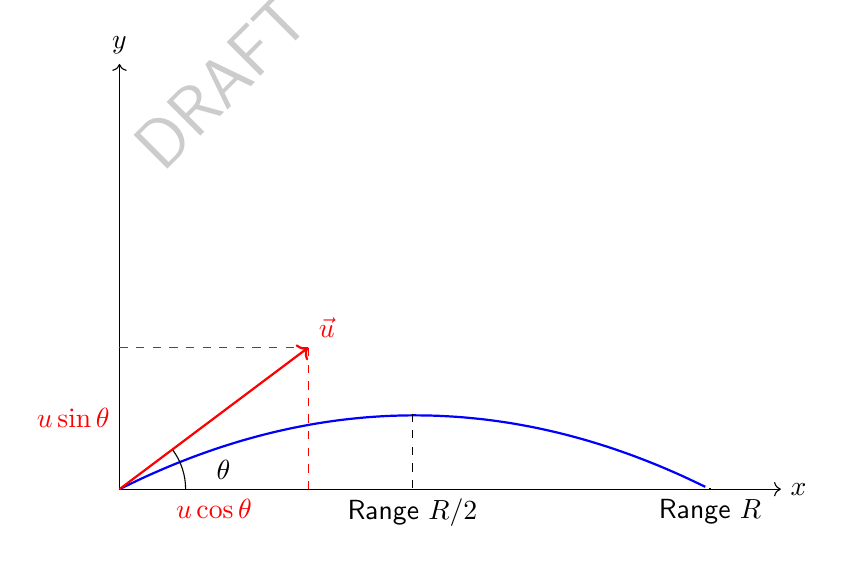
\begin{tikzpicture}[scale=1.2]
    % Axes
    \draw[->] (0,0) -- (7,0) node[right] {$x$};
    \draw[->] (0,0) -- (0,4.5) node[above] {$y$};

    % Parabolic trajectory
    \draw[thick,domain=0:6.2,smooth,variable=\x,blue] plot ({\x},{0.5*\x - 0.08*\x*\x});

    % Initial velocity vector
    \draw[->,red,thick] (0,0) -- (2,1.5) node[above right] {$\vec{u}$};

    % Components of initial velocity
    \draw[dashed,red] (2,0) -- (2,1.5);
    \draw[dashed,red] (0,1.5) -- (2,1.5);
    \node[below,red] at (1,0) {$u \cos \theta$};
    \node[left,red] at (0,0.75) {$u \sin \theta$};

    % Angle theta
    \draw (0.7,0) arc[start angle=0,end angle=36, radius=0.7];
    \node at (1.1,0.2) {$\theta$};

    % Labels
    \node[below left] at (0,0) {};

    % Apex (highest point)
    \draw[dashed] (3.1,0.8) -- (3.1,0);
    \node[below] at (3.1,0) {Range $R/2$};

    % Total range
    \draw[dashed] (6.25,0) -- (6.25,0.01);
    \node[below] at (6.25,0) {Range $R$};

  \end{tikzpicture}
\end{figure}

\begin{itemize}
  \item The initial velocity $u$ has horizontal component $u_x = u \cos \theta$ and vertical component $u_y = u \sin \theta$.
  \item The horizontal component of the velocity is given by $u_x = u \cos \theta$ and is constant throughout the motion.
  \item At the maximum height (the stationary point), the vertical velocity switches direction and becomes downwards from there on.
  \item There is only vertical acceleration on the object -- $g$ downward.
  \item The maximum height is given by
        $$h = \frac{u^2 \sin^2 \theta}{2g}$$
  \item The duration of the entire journey is the following, which is also twice the time to reach the maximum height:
        $$T = \frac{2u \sin \theta}{g}$$
\end{itemize}

\section{Types of Forces}

\subsection{Tension}

Tension is the force that arises in any body when it is stretched or
compressed.\lb
A tension force in a string is created when two forces are applied in opposite directions at the ends of the string. It acts along the length of the string, and always pulls away from the object tied to the string at either end -- never pushes.\lb
We normally assume that the string is massless and inextensible, and so the \hl{tension is the same throughout (at any point of) the string}.\lb
Consider the following situation where a mass $m$ is tied onto a string and is hanging from the ceiling.

\begin{figure}[H]
  \centering
  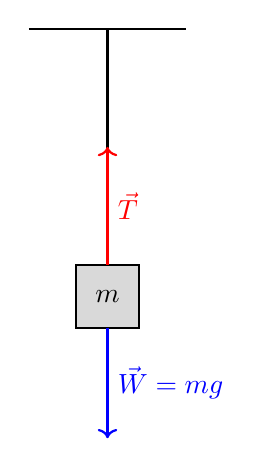
\begin{tikzpicture}
    % Ceiling
    \draw[thick] (-1, 0) -- (1, 0);

    % Rope
    \draw[thick] (0, 0) -- (0, -3);

    % Mass
    \draw[fill=gray!30, thick] (-0.4, -3) rectangle (0.4, -3.8);
    \node at (0, -3.4) {\( m \)};

    % Tension force arrow
    \draw[->, thick, red] (0, -3) -- (0, -1.5) node[midway, right] {\( \vec{T} \)};

    % Weight force arrow
    \draw[->, thick, blue] (0, -3.8) -- (0, -5.2) node[midway, right] {\( \vec{W} = mg \)};
  \end{tikzpicture}
  \caption{A mass \( m \) hanging from a rope with tension \( \vec{T} \) and weight \( \vec{W} = mg \).}
\end{figure}
\bigskip
It is said that there is a tension $T = W = mg$ in the string. This tension is upward so as to balance the weight of the mass.

\pagebreak

\subsection{Drag Force}

The drag force in a fluid is given by:
$$F_d = 6\pi \eta r v$$
where:
\begin{itemize}
  \item $F_d$ is the drag force
  \item $\eta$ is the viscosity of the fluid
  \item $r$ is the radius of the object
  \item $v$ is the velocity of the object
\end{itemize}

It is in the opposite direction of the velocity vector.\lb
An explanation on the forces acting on a skydiver can be asked in exams; let us consider the scenario with respect to a velocity/time graph
\img{material/terminalvgraph.png}{0.75}{Velocity/time graph of a skydiver}{skydiver}

\begin{enumerate}
  \item When the skydiver jumps out of the plane, immediately there is a \hl{constant gravitational force} acting on them, initially giving a downward acceleration of $g$.
  \item As the skydiver accelerates downwards, the \hl{drag force opposing their motion increases} because the velocity is increasing and the \hl{skydiver hits the air particles with more force} (so greater resistance upwards, by N$^{3\text{rd}}$).
  \item The \hl{drag force continues to increase} until it is equal to the gravitational force, at which point the \hl{net force acting on the skydiver is zero}, and a terminal velocity is reached.
  \item The instant the skydiver opens their parachute, the \hl{drag force increases significantly}, and the drag force now is much greater than the gravitational force, causing the skydiver to \hl{decelerate} rapidly.
  \item With decreasing velocity, the \hl{drag force also decreases} until it is equal to the gravitational force again, at which point the skydiver reaches a \hl{new, lower terminal velocity.}
\end{enumerate}

\pagebreak

\subsection{Buoyancy Force}

The buoyancy force exerted by a fluid on an object is given by:
$$F_b = \rho g V$$
where:
\begin{itemize}
  \item $F_b$ is the buoyancy force
  \item $\rho$ is the density of the fluid
  \item $g$ is the acceleration due to gravity
  \item $V$ is the volume of the fluid displaced
\end{itemize}

This force is always directed upwards, against the force of gravity. It is worth noting that, when the object is fully submerged, the volume of the fluid displaced is equal to the volume of the object.\lb
A useful ratio is
$$\frac{\rho_\text{obj}}{\rho_\text{fluid}} = \text{fraction of the object submerged}$$
where:

This allows us to find the terminal velocity $v_0$ of an object of volume $V$ and density $\rho_\text{obj}$ falling through a fluid of density $\rho_\text{fluid}$:
\begin{align*}
  F_b + F_d = F_g                                               \\
  \rho_\text{fluid} g V + 6\pi \eta r v_0 = \rho_\text{obj} g V \\
  v_0 = \frac{\left(\rho_\text{obj} - \rho_\text{fluid}\right) g V}{6\pi \eta r}
\end{align*}


\pagebreak

\subsection{Frictional Force}

The frictional force is given by:
$$F_f = \mu F_n$$
where:
\begin{itemize}
  \item $F_f$ is the frictional force
  \item $\mu$ is the coefficient of friction
        \begin{itemize}
          \item The static coefficient $\mu = \mu_s$ is used when the object is at rest relative to the surface.
          \item The kinetic coefficient $\mu = \mu_d$ is used when the object is in motion relative to the surface.
        \end{itemize}
\end{itemize}

It then follows that the maximum force along the surface before the object starts moving is given by:
$$F_{f, \text{max}} = \mu_s F_n$$

Exerting a force greater than this limit will cause the object to start moving, in which case, the frictional force now must use the kinetic coefficient.\lb
It must be noted that $\mu_s > \mu_d$, and so the static frictional force is always greater than the kinetic frictional force.\lb

\pagebreak

\subsection{Spring Force}

The spring force is given by:
$$F_s = -kx$$
where:
\begin{itemize}
  \item $F_s$ is the spring force
  \item $k$ is the spring constant
  \item $x$ is the displacement from the equilibrium position
\end{itemize}
The negative sign indicates that the force is always directed opposite to the displacement.


\pagebreak

\section{Circular Motion}

The equations are
\begin{itemize}
  \item Linear acceleration: $a = v\omega = \dfrac{v^2}{r} = \omega^2r$ is the centripetal acceleration, directed inwards towards the center of the circle.
  \item Linear speed: $v = \dfrac{2\pi r}{T} = r\omega = 2\pi r f$
  \item Angular speed: $\omega = \dfrac{2\pi}{T}$
  \item Frequency: $f = \dfrac{1}{T}$
\end{itemize}

It must be noted that, when drawing free body diagrams, the centripetal force is \hl{not a type of force in itself}, but rather a net force acting on the object, and so should not be drawn. We will practice with this in the Exam Questions section later on.\lb
There are a few scenarios that we investigate in IB questions; below is the list identifying the force providing the centripetal force.
\begin{table}[H]
  \centering
  \begin{tabular}{|c|c|}
    \hline
    \rowcolor{BlueGreen!35!white}
    \textbf{Scenario}                                  & \textbf{Centripetal Force}      \\ \hline
    Car at a roundabout                                & Frictional force                \\
    Object on a string rotating in a horizontal circle & Horizontal component of tension \\
    Bicycle on a banked curve                          & Normal force                    \\
    Satellites in orbit                                & Gravitational force             \\
    Rotor ride                                         & Normal reaction force           \\\hline
  \end{tabular}
\end{table}

\pagebreak

\subsection{Vertically Rotating Object on a String}

Consider a mass attached to a string rotating in a vertical circle.

\img{material/circular.png}{0.4}{Free body diagram of a mass attached to a string}{circular}

The diagram shows the forces acting on an object at four different points.


\pagebreak


\subsection{Turning without Slipping}

Consider a car turning around a corner, whose path is modelled by a circle of radius $r$.

\begin{minipage}{0.35\textwidth}
  \centering
  \img{material/turn1.png}{1}{Car turning around a corner}{carturn}
\end{minipage}\hspace{0.1\textwidth}%
\begin{minipage}{0.55\textwidth}
  \centering
  \img{material/turn2.png}{1}{Forces acting on a car turning around a corner}{carturnforces}
\end{minipage}


Suppose road has a static friction coefficient $\mu_s$ and the car has a mass $m$. The car is moving with a speed $v$ and the radius of the turn is $r$. The forces acting on the car are:
\begin{itemize}
  \item Vertically: The weight of the car $mg$ acting downwards and the normal force $F_n = mg$ acting upwards.
  \item Horizontally: The frictional force $F_f$ acting towards the center of the circle.
\end{itemize}

The common problem in IB questions is to find the maximum speed at which the car can turn without slipping. This is where the frictional force does not surpass the maximum static frictional force. This means
\begin{align*}
  F_c \le F_\text{f, static}  \\
  \frac{mv^2}{r} \le \mu_s mg \\
  v^2 \le \mu_s g r           \\
  v \le \sqrt{\mu_s g r}
\end{align*}

\pagebreak

\subsection{Banking}

Suppose an object travelling on a curved path with radius $r$ banked at an angle $\theta$ to the horizontal. The free body diagram is as follows
\img{material/banking.png}{0.4}{Free body diagram of a banked curve}{banking}
\begin{itemize}
  \item The vertical component of the normal force $F_n$ is equal to the weight of the object $mg$, since the object is not accelerating vertically.
  \item The centripetal force is provided by the horizontal component of the normal force $F_n$, namely $N \sin \theta$.
\end{itemize}

\pagebreak

\subsection{Car over a Bridge/Hill}

What is the maximum speed at which a car can go over a bridge/hill of radius $r$ without losing contact with the road? The diagram is as follows.

\img{material/bridge.png}{0.4}{Car over a bridge}{bridge}
\begin{enumerate}
  \item The forces acting on the car are
        \begin{itemize}
          \item Downward weight $mg$
          \item Normal reaction force $F_n$ acting upwards
          \item The net force is the centripetal force
                $$F_c = \frac{mv^2}{r} = mg - F_n$$
          \item You might be tempted to think that $W = F_n$ -- this is not true. We are dealing with circular motion, so there must be a non-zero net force keeping the car in circular motion.

        \end{itemize}
  \item If, at any point, this normal force is zero, then the car will lose contact with the road. For this to happen, the normal reaction force must be $0$, giving
        \begin{align*}
          g & = \frac{v^2}{r} \\
          v & = \sqrt{gr}
        \end{align*}
\end{enumerate}

\section{Energy}

\begin{itemize}
  \item Kinetic energy: $E_K = \dfrac{1}{2}mv^2 = \dfrac{p^2}{2m}$
  \item Gravitational potential energy: $E_P = mgh$
  \item Elastic potential energy: $E_E = \dfrac{1}{2}kx^2$
  \item Work done: $W = Fd\cos \theta$
  \item Power: $P = \dfrac{W}{t} = Fv\cos \theta$
\end{itemize}

\subsection{Sankey Diagrams}

They are used for both energy and power. The rules of a Sankey diagram are as follows:
\begin{itemize}
  \item The diagram is drawn to scale with the width of the arrow being proportional to the amount of energy transfer it represents.
  \item Left to right: The energy input is on the left, and the energy output is on the right.
  \item Lost/wasted energy is directed downwards.
\end{itemize}

\img{material/sankey.png}{0.5}{Sankey diagram of a car}{sankey}

\section{Momentum}

Momentum, as an attribute of a body, is given as
$$p = mv$$
where:
\begin{itemize}
  \item $p$ is the momentum
  \item $m$ is the mass
  \item $v$ is the velocity
\end{itemize}

The momentum of a system is given by the sum of the momenta of all objects.\lb
The \textbf{impulse}, change in momentum, is given by:
$$\Delta p = F \Delta t = m(\Delta v)$$
The differential form (through the product rule) can be used when one or both of mass and velocity are changing:
$$\Delta p = \diff{(mv)}{t} = m \diff{v}{t} + v \diff{m}{t}$$
This is useful in situations such as rockets, where the mass is changing due to fuel consumption. When a rocket is travelling while expelling fuel, the total momentum of the fuel-rocket system is conserved. We will practice this later.

\pagebreak

\subsection{Collisions and Explosions}

In these cases, the total momentum of the system is conserved \hl{only if the net force acting on the system is 0}. Hence
$$\sum p_\text{before} = \sum p_{\text{after}}$$
Often times, these questions may involve looking at both components. It is important to know that the momentum is conserved in all directions, and so the momentum in the x-direction and y-direction are conserved separately, which can give us a system of equations to solve. We will practice later.\lb
For it to be an elastic collision, the kinetic energy must also be conserved. This means that
$$\sum E_{K, \text{before}} = \sum E_{K, \text{after}}$$
In a lot of questions, you'd be ask to determine whether the collision is elastic or inelastic. This can be done by checking if the kinetic energy before and after the collision is equal. If it is, then it is elastic, otherwise it is inelastic.\lb

\section{Exam Questions}

\subsection{MCQ \#1 -- Projectile}

A projectile is launched with an initial kinetic energy $E$. The initial horizontal and vertical components of velocity are equal. Air resistance is negligible.
What is the kinetic energy of the projectile at the highest point of the motion?

\begin{enumerate}[label=\Alph*.]
  \item zero
  \item $\dfrac{E}{4}$
  \item $\dfrac{E}{2}$
  \item $E$
\end{enumerate}

\begin{itemize}
  \item Both components have the same initial speed and this means that the KE is equally divided between the two components.
  \item Recall that the horizontal component of the velocity is constant, and so the horizontal component of the KE, namely $\dfrac{E}{2}$, remains constant.
  \item At the highest point, the vertical velocity and hence the vertical component of the KE is zero.
  \item So the total KE is equal to the horizontal component of the KE, which is $\dfrac{E}{2}$.
  \item \ans{C}
\end{itemize}

\let\oldsubsection\subsection
\renewcommand\subsection{\clearpage\oldsubsection}

\pagebreak

\subsection{MCQ \#2 -- Projectile}
A ball is thrown upwards at time $t = 0$. The graph shows the variation with time of the height of the ball. The ball returns to the initial height at time $T$.
\img{ex/1.png}{0.7}{Graph of height vs time}{heightvtime}
What is the height $h$ at time $t$?

\begin{enumerate}[label=\Alph*.]
  \item $\dfrac{1}{2}gt^2$
  \item $\dfrac{1}{2}gT^2$
  \item $\dfrac{1}{2}gT(T - t)$
  \item $\dfrac{1}{2}gt(T - t)$
\end{enumerate}

Walkthrough:
\begin{itemize}
  \item You could do this the hard way and use SUVAT. If you are satisfied with that, skip to the next question.
  \item Let us use a bit more of reasoning.
        \begin{enumerate}
          \item By the nature of the projectile motion, the graph of s/t has to be parabolic and thus a quadratic in $t$ (\outs{B}{C}, quadratics in $T$). In this case, it has roots $t = 0$ and $t = T$ (\ans{D}).

        \end{enumerate}
\end{itemize}

\pagebreak

\subsection{MCQ \#3 -- Two-Stage Motion}

An object is released from rest and slides down a frictionless ramp. The object then leaves the ramp and slides along a rough horizontal surface. The object stops in a distance along the ramp.

\img{ex/9.png}{0.7}{Sliding down a ramp}{ramp}

The coefficient of dynamic friction between the object and the rough horizontal surface is $\mu$.
What is the height of the ramp?

\begin{enumerate}[label=\Alph*.]
  \item $\mu g s$
  \item $\dfrac{s}{2g\mu}$
  \item $\dfrac{s}{\mu}$
  \item $s\mu$
\end{enumerate}

\begin{itemize}
  \item If we are smart enough we can already tell that A and B cannot be the answer, because their units are not consistent with the units of height.
  \item
\end{itemize}

\subsection{MCQ \#4 -- Momentum Conservation and Springs}
A spring of negligible mass is compressed and placed between two stationary
masses $m$ and $2m$. The spring is released so that
the masses move in opposite directions.\lb
What is $\dfrac{\text{KE of $m$}}{\text{KE of $2m$}}$?
\begin{enumerate}[label=\Alph*.]
  \item $\dfrac{1}{2}$
  \item $1$
  \item $2$
  \item $4$
\end{enumerate}

You may be tempted to use energy equations, but that wouldn't get you too far. We should use the conservation of momentum instead.
\begin{align*}
  0                        & = m v_1 - 2m v_2 \\
  \frac{v_1}{v_2}          & = 2              \\
  \frac{mv_1^2}{(2m)v_2^2} & = 2              \\
\end{align*}

\ans{C}

\subsection{MCQ \#5 -- Momentum Conservation and Springs (2)}

Masses X and Y rest on a smooth horizontal surface and are connected by a massless spring. The mass of X is 3.0 kg and the mass of Y is 6.0 kg. The masses are pushed toward each other until the elastic potential energy stored in the spring is 1.0 J.

\img{ex/12.png}{0.3}{Masses connected by a spring}{spring}

The masses are released. What is the maximum speed reached by mass Y?

\begin{enumerate}[label=\Alph*.]
  \item 0.11
  \item 0.33
  \item 0.45
  \item 0.66
\end{enumerate}

\begin{itemize}
  \item First, we know momentum is conserved, so
        $$3v_X = 6v_Y \iff v_X = 2v_Y$$
  \item Then, the maximum speed is achieved when all the elastic potential energy is just transferred to the kinetic energy of both masses, so
        \begin{align*}
          \frac{1}{2}(3)(v_X^2) + \frac{1}{2}(6)(v_Y^2) & = 1 \\
        \end{align*}
  \item We substitute the relation between $v_X$ and $v_Y$ in to obtain
        $$6v_Y^2 + 3v_Y^2 = 1$$
  \item And finally
        $$v_Y^2 = \frac{1}{9} \implies v_Y = \frac{1}{3}$$
  \item \ans{B}
\end{itemize}

\subsection{MCQ \#6 -- Circular Motion}

Two masses $M$ and $m$ are connected by a string that runs without friction through a stationary tube. Mass rotates at constant speed in a horizontal circle of radius 0.25 m. The weight of provides the centripetal force for the motion of. The time period for the rotation of m is 0.50 s.\lb
What is $\dfrac{M}{m}$ approximately equal to?

\begin{enumerate}[label=\Alph*.]
  \item 1
  \item 2
  \item 4
  \item 8
\end{enumerate}

\begin{itemize}
  \item Let's first work with the time period condition
        $$Tv = 2\pi r \iff v = \frac{2\pi (0.25)}{\frac{T}{2}} = \pi$$
  \item We know that the centripetal force is in fact the weight of the $M$ mass, so
        \begin{align*}
          \frac{mv^2}{r} & = Mg                          \\
          \frac{M}{m}    & = \frac{v^2}{g r}             \\
                         & = \frac{4\pi^2}{g}            \\
                         & \approx \frac{4\times 3^2}{9} \\
                         & \approx 4
        \end{align*}
  \item \ans{C}
\end{itemize}

\subsection{MCQ \#7 -- Force Pairs and Logic}

The magnitude of the resultant of two forces acting on a body is 12 N. Which pair of forces acting on the body can combine to produce this resultant?
\begin{enumerate}[label=\Alph*.]
  \item 1 N and 2 N
  \item 1 N and 14 N
  \item 5 N and 6 N
  \item 6 N and 7 N
\end{enumerate}
Solution
\begin{itemize}
  \item The key idea is that the forces do not have to be acting along the same axis, so there can be an angle between them, that is why no pair sum up or subtract to 12 N.
  \item However, what we do know is that the absolute minimum resultant of a force pair is $|F_1 - F_2|$, and the maximum resultant is $F_1 + F_2$.
  \item We want the pair to be such that
        $$|F_1 - F_2| \le 12 \le F_1 + F_2$$
  \item Only the fourth satisfies this condition. \ans{D}
\end{itemize}


\subsection{Misc \#1 -- Pulley}

A student uses a load to pull a box up a ramp inclined at 30°. A string of constant length and negligible mass connects the box to the load that falls vertically. The string passes over a pulley that runs on a frictionless axle. Friction acts between the base of the box and the ramp. Air resistance is negligible.

\img{ex/2.png}{0.7}{Pulley system}{pulley}

The load has a mass of 3.5 kg and is initially 0.95 m above the floor. The mass of the box is 1.5 kg.\lb
The load is released and accelerates downwards.

\begin{enumerate}[label=(\alph*)]
  \item Outline \textbf{two} differences between the momentum of the box and the momentum of the load at the same instant.
        \begin{itemize}
          \item The momentum of the box is less than the momentum of the load because they have the same velocity, but the load has a greater mass.
          \item The directions of motion are different.
        \end{itemize}
  \item The vertical acceleration of the load downwards is $\SI{2.4}{\m\per\s\squared}$.

        Calculate the tension in the string.
        \begin{itemize}
          \item We start by looking at the forces acting on the load. Let us draw the following free body diagram

                \begin{figure}[H]
                  \centering
                  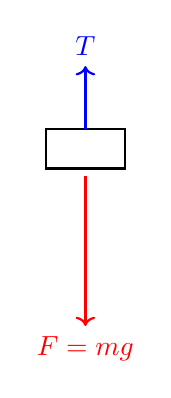
\begin{tikzpicture}
                    % Draw the object (a box)
                    \draw[thick] (-0.5,0) rectangle (0.5,0.5);

                    % Tension force (upwards)
                    \draw[->, thick, blue] (0,0.5) -- (0,1.3) node[above] {\( T \)};

                    % Force = ma (downwards)
                    \draw[->, thick, red] (0,-0.1) -- (0,-2) node[below] {\( F = mg \)};


                  \end{tikzpicture}
                \end{figure}
          \item We are given the actual downward acceleration of the load, which corresponds to its resultant force. Hence
                \begin{align*}
                  ma & = mg - T                  \\
                  T  & = m(g-a)                  \\
                     & = 3.5 \times (9.81 - 2.4) \\
                     & = \SI{26}{\newton}
                \end{align*}
        \end{itemize}
  \item \begin{enumerate}[label=(\roman*)]
          \item Show that the speed of the load when it hits the floor is about $\SI{2.1}{\m\per\s}$
                \begin{align*}
                  v & = \sqrt{u^2 + 2as}                    \\
                    & = \sqrt{0 + 2 \times 2.4 \times 0.95} \\
                    & = \SI{2.14}{\m\per\s}
                \end{align*}
          \item The radius of the pulley is 2.5 cm. Calculate the angular speed of rotation of the pulley as the load hits the floor. State your answer to an appropriate number of significant figures.
                \begin{align*}
                  \omega & = \frac{v}{r} = \frac{2.1}{0.025} = 84
                \end{align*}
        \end{enumerate}
  \item After the load has hit the floor, the box travels a further 0.35 m along the ramp before coming to rest. Determine the average frictional force between the box and the surface of the ramp.
        \begin{itemize}
          \item We must recognize that the only thing that can bring the box to rest is the frictional force $F_f$ opposing its motion. But there is an issue of components here so let us first visualise the situation with a free body diagram (our favourite)
                \begin{figure}[H]
                  \centering
                  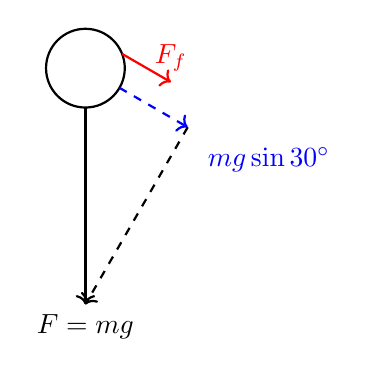
\begin{tikzpicture}
                    \draw[thick] (0,0) circle (0.5);

                    \draw[->,thick,dashed,blue] (0.433013, -0.25) -- (1.29904, -0.75) node[below right=5pt] {\( mg\sin 30\degsym \)};

                    \draw[->,thick,dashed] (1.29904, -0.75) -- (0, -3) node[below] {};


                    \draw[->, thick] (0,-0.5) -- (0,-3) node[below] {\( F = mg \)};

                    \draw[->,thick,red] (0.46614, 0.18088) -- (1.08569,-0.17683) node[above] {$F_f$};


                  \end{tikzpicture}
                \end{figure}
          \item Wee see that the resultant force acting on the box to bring it to rest is the following sum
                $$ma = F_f + mg\sin 30\degsym \iff F_f  = m(a - g\sin 30\degsym)$$
          \item We are given $m$ but $a$ is still unknown at this point. We need another equation.
          \item We know that the force as a result of this net acceleration $a$ brings the object to rest in 0.35 m. We can use SUVAT, since the acceleration is constant.

                \begin{align*}
                  a & = \frac{v^2 - u^2}{2s}            \\
                    & = \frac{0 - 2.1^2}{2 \times 0.35} \\
                    & = 6.3
                \end{align*}
          \item Now we are ready to substitute this value of $a$ into the equation for $F_f$.
                \begin{align*}
                  F_f & = m(a - g\sin 30\degsym)   \\
                      & = 1.5 \times (6.3 - 4.905) \\
                      & = \SI{2.1}{\newton}
                \end{align*}



        \end{itemize}
  \item The student then makes the ramp horizontal and applies a constant horizontal force to the box. The force is just large enough to start the box moving. The force continues to be applied after the box begins to move.

        \img{ex/3.png}{0.35}{Box on a horizontal ramp}{boxhorizontal}

        Explain, with reference to the frictional force acting, why the box accelerates once
        it has started to move.
        \begin{enumerate}[label=\arabic*.]
          \item $\mu_s > \mu_d$
          \item for the object to start moving, the applied force must be greater than the maximum static frictional force.
          \item Once the object starts moving, the applied force remains the same but the frictional force is now the kinetic frictional force, which is less than the static frictional force. Thus, the forces are now unbalanced. $F = ma$, so there is an acceleration.
        \end{enumerate}
\end{enumerate}

\subsection{Misc \#2 -- Passing over a Net}

A student strikes a tennis ball that is initially at rest so that it leaves the racquet at a
speed of $\SI{64}{\m\per\s}$. The ball has a mass of 0.058 kg and the contact between the ball and the racquet lasts for 25 ms.

The student strikes the tennis ball at point P. The tennis ball is initially directed at an angle of 7.00$\degsym$ to the horizontal.

\img{ex/4.png}{0.8}{Tennis ball hitting a racquet}{tennisball}

The following data are available.
\begin{itemize}
  \item Height of P = $\SI{2.80}{\m}$
  \item Distance of student from net = $\SI{11.9}{\m}$
  \item Height of net = $\SI{0.910}{\m}$
  \item Initial speed of tennis ball = $\SI{64}{\m\per\s}$
\end{itemize}

\begin{enumerate}[label=(\alph*)]
  \item \begin{enumerate}[label=(\roman*)]
          \item Calculate the average power delivered to the ball during the impact.
                \begin{align*}
                  P & = \frac{E_K}{t}                  \\
                    & = \frac{\frac{1}{2}mv^2}{t}      \\
                    & = \frac{0.5(0.058)(64^2)}{0.025} \\
                    & = 4751.36                        \\
                    & \approx \SI{4800}{\watt}
                \end{align*}
        \end{enumerate}
  \item Show that the tennis ball passes over the net.
        \begin{itemize}
          \item We must first determine the time it takes the ball to reach the net horizontally.
                \begin{align*}
                  11.9 = 64\cos(7\degsym) t \implies t = 0.187...
                \end{align*}
          \item We then determine its vertical position at this time. If it is greater than the height of the net, then it passes over it.
                \begin{align*}
                  \Delta y & = -64\sin(7\degsym)(0.187) - \frac{1}{2}(9.8)(0.187^2) \\
                           & = -1.63                                                \\
                  y        & = 2.8 - 1.63                                           \\
                           & = 1.17 \ge0.91
                \end{align*}
          \item Hence, it will pass over the net.
        \end{itemize}
  \item The student models the bounce of the tennis ball to predict the angle $\theta$ at which the ball leaves a surface of clay and a surface of grass.

        \img{ex/5.png}{0.9}{Tennis ball bouncing off a surface}{tennisballbounce}
        The model assumes
        \begin{itemize}
          \item during contact with the surface the ball slides.
          \item the sliding time is the same for both surfaces.
          \item the sliding frictional force is greater for clay than grass.
          \item the normal reaction force is the same for both surfaces.
        \end{itemize}
        Predict for the student's model, without calculation, whether $\theta$ is greater for a clay surface or for a grass surface.
        \begin{itemize}
          \item The normal force is the same so the vertical component of the velocity is the same for both.
          \item Clay has a greater frictional force than grass, so the horizontal component of the velocity is less for clay.
          \item Hence, the angle $\theta$ is greater for clay than for grass.
        \end{itemize}
\end{enumerate}


\subsection{Tension \#1}

A bird of weight $W$ sits on a thin rope at its midpoint. The rope is almost horizontal and has negligible mass.

\img{ex/6.png}{0.5}{Bird on a rope}{birdrope}

The tension in the rope is
\begin{enumerate}[label=\Alph*.]
  \item less than $\dfrac{W}{2}$
  \item equal to $\dfrac{W}{2}$
  \item between $\dfrac{W}{2}$ and $W$
  \item greater than $W$
\end{enumerate}

We can draw the free body diagram to visualise the problem, bearing in mind that \hl{we label the tensions at the ends of the string}.

\begin{figure}[H]
  \centering
  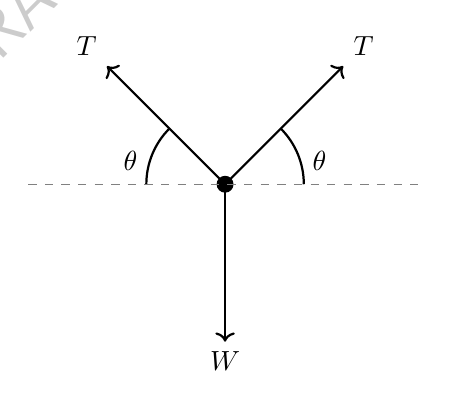
\begin{tikzpicture}
    \filldraw[black] (0,0) circle (0.1);

    \draw[->, thick] (0,0) -- (0,-2) node[below] {$W$};

    \draw[->, thick] (0,0) -- (1.5,1.5) node[above right] {$T$};
    \draw[->, thick] (0,0) -- (-1.5,1.5) node[above left] {$T$};

    \draw[thick] (1,0) arc[start angle=0,end angle=45,radius=1];
    \node at (1.2,0.3) {$\theta$};

    \draw[thick] (-1,0) arc[start angle=180,end angle=135,radius=1];
    \node at (-1.2,0.3) {$\theta$};

    \draw[dashed, gray] (-2.5,0) -- (2.5,0);
  \end{tikzpicture}
\end{figure}
Since the object in equilibrium, the vertical components of the forces must balance, and so
$$2T\sin \theta = W\implies T = \frac{W}{2\sin\theta}$$
We are told that the rope is almost horizontal, which means that $\theta$ is very small. Recall that $$\lim\limits_{\theta \to 0} \sin \theta = 0$$
So $T$ is very large, and hence the tension in the rope is greater than $W$.


\subsection{Bi-body Movement \#1}

A block of mass 45 kg is placed on a horizontal table.
There is no friction between the block and the table.\lb
An object of mass 15 kg is placed on top of the block.\lb
A force $F$ acts on the block so that it accelerates. The acceleration of the object and the acceleration of the block are the same so that they do not move relative to each other.

\img{ex/7.png}{0.5}{Block on a table}{blocktable}

The coefficient of static friction between the block and the object is 0.60.

\begin{enumerate}[label=(\alph*)]
  \item State the nature and direction of the force that accelerates the 15 kg object.
        \begin{itemize}
          \item Static friction
          \item to the right.
        \end{itemize}
  \item Determine the largest magnitude of $F$ for which the block and the object do not move relative to each other.
        \begin{itemize}
          \item If we want the two objects to move together, they must have the same acceleration. Let's call this mutual resultant acceleration $a$. Then
                $$F = 60a$$
          \item The frictional force is the only force acting on the 15 kg object, and so
                $$F_f = ma = 15a$$
          \item We can now compute the acceleration of the 15 kg object, since we know the coefficient of static friction.
                \begin{align*}
                  \mu_s F_N & = 15a                                 \\
                  a         & = \frac{\mu_s F_N}{15}                \\
                            & = \frac{0.6 \times 15 \times 9.8}{15} \\
                            & = 0.6\times 9.8
                \end{align*}
          \item We can now substitute this into $F = ma$ to obtain $$F = 60\times 0.6\times 9.8 = 352.8 \approx \SI{350}{\newton}$$
        \end{itemize}
\end{enumerate}

\subsection{Bi-body Movement \#2}

The diagram shows two blocks of mass $m$ and $M$ in contact on a frictionless surface. A force $F$ is applied on the block of mass and causes the blocks to move with an acceleration.

\img{ex/10.png}{0.8}{Two blocks on a table}{twoblocks}

What is the force that the block of mass $M$ is exerting on the block of mass $m$?

\begin{itemize}
  \item We begin my looking at the entire system. The entire body is travelling with an acceleration $a$, and so the net force acting on it is given by (this is the $F$ force that we are exerting)
        $$F = (m + M)a$$
  \item We now zoom in on the single $m$ mass and drawing its free body diagram.
  \item The force $N$ indicates what the $M$ block exerts on the $m$ block, which is what we are looking for.
\end{itemize}

\begin{figure}[H]
  \centering
  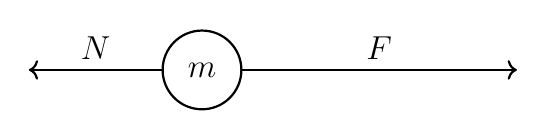
\begin{tikzpicture}

    % Draw the body (circle)
    \draw[thick] (0,0) circle (0.5);
    \node at (0,0) {\large $m$};

    % Draw the larger force to the right (F)
    \draw[->, thick] (0.5,0) -- (4,0) node[midway, above] {\large $F$};

    % Draw the smaller force to the left (F')
    \draw[->, thick] (-0.5,0) -- (-2.2,0) node[midway, above] {\large $N$};

  \end{tikzpicture}
\end{figure}

\begin{itemize}
  \item The mass is travelling with an acceleration $a$, and so the net force acting on it is given by
        $$F - N = ma \iff N = F - ma$$
  \item We substitute $F = (m+M)a$ back in the above to obtain
        \begin{align*}
          N & = ma + Ma - ma \\
            & = Ma
        \end{align*}
\end{itemize}

\subsection{Bi-body Movement \#3}

X and Y are two objects on a frictionless table connected by a string. The mass of X is 2 kg and the mass of Y is 4 kg. The mass of the string is negligible. A constant horizontal force of 12 N acts on Y.

\img{ex/11.png}{0.5}{Two blocks connected by a string}{twoblocks2}

What are the acceleration of Y and the magnitude of the tension in the string?

\begin{itemize}
  \item Again, we begin by looking at the entire system first: The net force acting on the $4 + 2 = 6$ kg system is 12, which means they both accelerate at \hlans{$a = 2$}.
  \item We now zoom in on the $4$ kg mass because it has both the tension and $12$N force acting on it, which can provide more useful information.
        \begin{align*}
          F_\text{net} & = 12 - T \\
          F_\text{net} & = ma = 8 \\
          T            & = 4
        \end{align*}
  \item Hence, \hlans{$T = 4$}
\end{itemize}

At this point, you should be able to see a pattern:
\begin{enumerate}
  \item Look at the entire system as a whole, often, this is the mutual acceleration.
  \item Then, focus on one of the masses, and draw the free body diagram.
  \item You should get a set of equations that, upon substitution, will yield the answer.
\end{enumerate}


\subsection{2D Momentum Conservation}

Ball A, moving in a horizontal direction at an initial speed of $\SI{2.0}{\m\per\s}$ collides with a stationary ball B of the same mass. After the collision, ball A moves at a speed of $\SI{1.0}{\m\per\s}$ at an angle of 45° to the original direction of motion.

\img{ex/8.png}{0.5}{Ball A colliding with ball B}{ballcollision}

\begin{enumerate}[label=(\alph*)]
  \item Calculate the vertical component of the velocity of ball B after the collision.
        \begin{align*}
          p_y \text{ before} = p_y \text{ after} = 0 \\
          v_\text{B, y} = \frac{1}{\sqrt{2}} \approx 0.71
        \end{align*}
  \item Determine the angle $\theta$ that the velocity of ball B makes with the initial direction of motion of ball A.
        \begin{align*}
          p_x \text{ before} = p_x \text{ after}                                       \\
          2 = v_\text{B, x} + 1\cos(45\degsym)                                         \\
          v_\text{B, x} = 2 - \frac{1}{\sqrt{2}} \approx 1.29                          \\
          \theta = \arctan\left(\frac{v_\text{B, y}}{v_\text{B, x}}\right) = 29\degsym \\
        \end{align*}
  \item Predict whether the collision is elastic
        \begin{itemize}
          \item Initial kinetic energy = $\frac{1}{2}mv^2 = \frac{1}{2}m(2^2) = 2m$
          \item Final total KE is
                \begin{align*}
                          & \frac{1}{2}m(1^2) + \frac{1}{2}m\left(\frac{0.71}{\sin(29\degsym)}\right) \\
                  \approx & 1.6m < 2m
                \end{align*}
          \item Hence, the collision is inelastic.
        \end{itemize}
\end{enumerate}



\end{document}